\documentclass[10pt,a4paper]{article}
\usepackage[utf8]{inputenc}
\usepackage{graphicx}
\author{Ken LE PRADO}
\title{Banc de test Modbus}
\begin{document}

\section{Introduction}

Modbus est un protocole réseau de SCADA notamment implémenté par des industriels tels que Schneider Electrics.
L'apprentissage et les tests sur le protocole Modbus est impensable sur un environnement réel, aussi, l'utilisation d'un banc de tests est une évidence.

Des bancs de tests réels existent mais sont relativement co\^uteux et peux flexibles. Ce document décrit la réalisation d'un banc de tests à base de briques Lego programmables (Lego Mindstorms EV3).

\section{Description générale}
L'objectif du banc de test est de mettre à disposition des éléments indépendants Management Terminal Unit (MTU) , Remote Terminal Unit (RTU)  qui communiquent entres eux à travers le protocole Modbus/TCP.

Le protocole utilisé par les RTU avec les capteurs ou les moteurs est I2C. Celui-ci est imposé par la brique Lego utilisée, et ne rentrera pas en considération.

La maquette choisie est celle d'un pont levant précédé par un ou plusieurs péages. Ces éléments (RTU) ne communiquent pas entre eux. Seul le centre de contr\^ole (ou MTU) lit l'état des RTU et modifie leurs registres.
L'Interface Homme-Machine (IHM) affiche l'état des valeurs récupérées et permet de modifier les registres.

La technologie utilisée est le framework Lejos\footnote{http://www.lejos.org}. Ce produit libre met à disposition un framework en Java pour l'IDE Eclipse permettant de développer simplement des applications pour Lego Mindstorms). Lejos met également à disposition une distribution Linux permettant d'éxécuter les applications développées.
Les communications Modbus sont gérées grâce à la librairie Jamod\footnote{http://jamod.sourceforge.net}. Cette librairie a été modifiée afin d'implémenter les fonctions de diagnostique de Modbus(code fonction 43).

Au niveau physique, les éléments sont reliés entre eux par USB, Bluetooth (PAN) ou WIFI.

\begin{center}
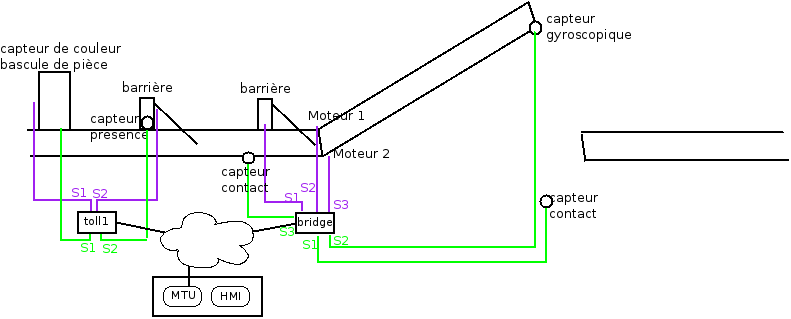
\includegraphics[scale=0.4]{schema_peage-pont.png}
\end{center}

\section{RTU}

Chaque RTU hérite d'une classe Device décrivant les fonctions essentielles de chaque RTU ().
Un péage ou un pont étend la classe Device\footnote{La documentation complète est disponible au format javadoc} permettant facilement de définir un nouveau type de composant.

\begin{center}
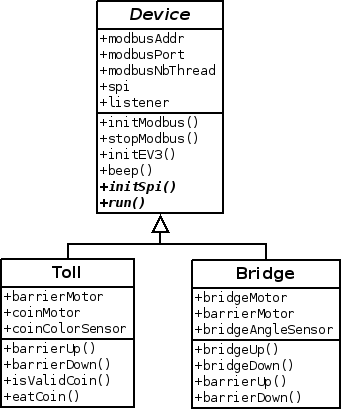
\includegraphics[scale=0.5]{Device_class.png}
\end{center}



\subsection{Péage}

Le système de péage présente l'intérêt d'être simple et reproductible sur le banc de test (en réel ou simulé).
Une version simulée (entièrement sur PC) est développée.

\begin{center}
\includegraphics[scale=0.2]{peage.jpg}
\end{center}

Les registres entretenus par le péage sont :

\begin{tabular}{|c|c|l|l|}
\hline 
\textbf{Type} & \textbf{Ref} & \textbf{Nom} & \textbf{Description} \\ 
\hline 
Input register & 0 & PIECE\_COLOR & Valeur du capteur de couleur de pièce \\ 
\hline 
Input register & 1 & CAR\_TOUCH & Valeur du capteur de passage de voiture \\ 
\hline 
Input register & 2 & KEY\_PRESS & Valeur du bouton pressé sur la brique EV3 \\ 
\hline 
Register & 0 & NAME\_ID & Identifiant de la barrière de péage \\ 
\hline 
Register & 1 & NB\_CARS & Nombre de véhicule ayant transités \\ 
\hline 
Register & 2 & NB\_COINS & Nombre de pièces valides avalées \\ 
\hline 
Coil & 0 & ACTIVE & Péage actif/non actif \\ 
\hline 
Coil & 1 & FREE & Péage gratuit/paiement activé \\ 
\hline 
Discrete Input & 0 & BARRIER & Position de la barrière (true = ouverte) \\ 
\hline 
\end{tabular} 

L'automate du péage décrit les états suivants :
TODO : Ajoute les états

\subsection{Pont levant}
Le pont levant permet de présenter un élément dont la sûreté de fonctionnement joue un r\^ole important, et donc les conséquences sont visibles immédiatement.

\begin{center}
\includegraphics[scale=0.2]{pont.jpg}
\end{center}

Les registres entretenus par le pont sont :

\begin{tabular}{|c|c|l|l|}
\hline 
\textbf{Type} & \textbf{Ref} & \textbf{Nom} & \textbf{Description} \\ 
\hline 
Input register & 0 & CAR\_PASSAGE & Valeur du capteur de passage de véhicule \\ 
\hline 
Input register & 1 & KEY\_PRESS & Valeur du bouton de l'EV3 pressé \\ 
\hline 
Input register & 2 & BRIDGE\_ANGLE & Valeur du capteur gyroscopique sur le tablier du pont (angle d'incidence du tablier) \\ 
\hline 
Input register & 3 & BOAT\_PASSAGE & Valeur du capteur de présence de bateau \\ 
\hline 
Register & 0 & NAME\_ID & Identifiant du pont \\ 
\hline 
Register & 1 & NB\_CARS & Nombre de véhicule ayant transités \\ 
\hline 
Coil & 0 & ACTIVE & Péage actif/non actif \\ 
\hline 
Coil & 1 & BRIDGE\_MOVE & Mouvement du péage demandé \\ 
\hline 
Coil & 2 & BRIDGE\_RAISE & Mouvement vers le haut ou vers le bas \\
\hline 
Coil & 3 & BARRIER\_OPENED & Position de la barrière \\ 
\hline 
Discrete Input & 0 & BARRIER & Position de la barrière (true = ouverte) \\ 
\hline 
Discrete Input & 1 & WAITING\_BOAT & Un bateau est-il en attente \\ 
\hline 
Discrete Input & 2 & BRIDGE\_UP & Le pont est-il levé\\ 
\hline 
\end{tabular} 

TODO : Ajoute les états

\section{centre de contrôle}
Le centre de contrôle désigne à la fois le MTU et l'IHM. Il assure le rôle de master dans les communications Modbus afin d'entretenir les états des registres des RTU et de les présenter à l'opérateur.

TODO : Ajouter un screenshot


\section{Appréciation du banc de test}

Ce banc de test implémente Modbus et permet d'effectuer des tests sur la sécurité du protocole.

La robustesse de l'implémentation est à améliorer, mais ne fait l'objet de l'étude.

\end{document}